\documentclass{article}

\usepackage{pgf}
\usepackage{tikz}
\usetikzlibrary{arrows,automata}
\usepackage[latin1]{inputenc}
\begin{document}
% sources:
% http://www.texample.net/tikz/examples/state-machine/
% http://martin-thoma.com/how-to-draw-a-finite-state-machine/

%\begin{tikzpicture}[->,>=stealth',shorten >=1pt,auto,node distance=2.8cm,
%                    semithick]
%  \tikzstyle{every state}=[fill=red,draw=none,text=white]
%
%  \node[initial,state] (A)                    {$q_a$};
%  \node[state]         (B) [above right of=A] {$q_b$};
%  \node[state]         (D) [below right of=A] {$q_d$};
%  \node[state]         (C) [below right of=B] {$q_c$};
%  \node[state]         (E) [below of=D]       {$q_e$};
%
%  \path (A) edge              node {0,1,L} (B)
%            edge              node {1,1,R} (C)
%        (B) edge [loop above] node {1,1,L} (B)
%            edge              node {0,1,L} (C)
%        (C) edge              node {0,1,L} (D)
%            edge [bend left]  node {1,0,R} (E)
%        (D) edge [loop below] node {1,1,R} (D)
%            edge              node {0,1,R} (A)
%        (E) edge [bend left]  node {1,0,R} (A);
%\end{tikzpicture}

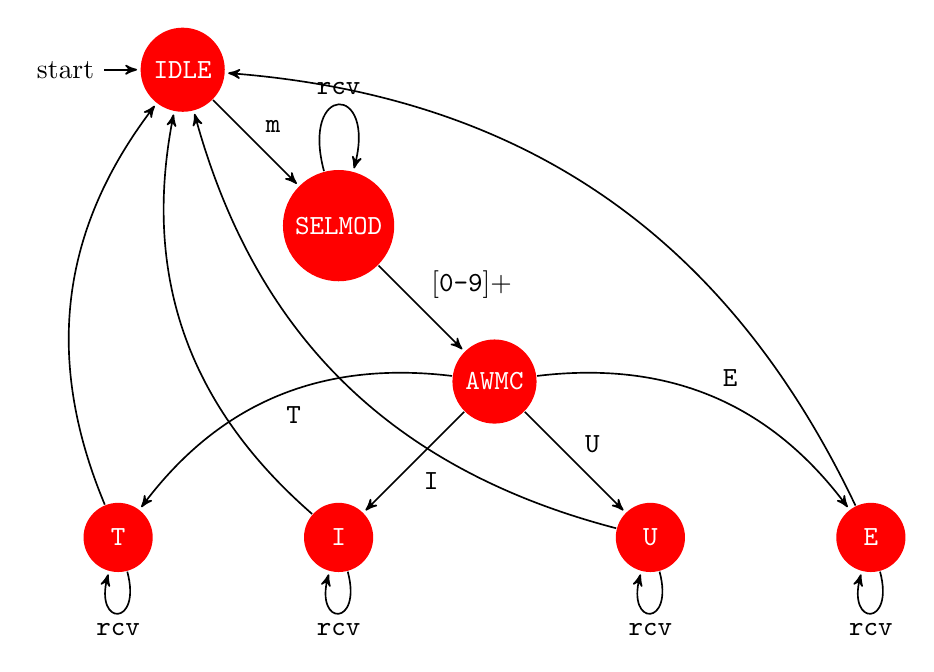
\begin{tikzpicture}[->,>=stealth',shorten >=1pt,auto,node distance=2.8cm,
                    semithick]
  \tikzstyle{every state}=[fill=red,draw=none,text=white]

  \node[initial,state] (A)                    {\texttt{IDLE}};
  \node[state]         (B) [below right of=A] {\texttt{SELMOD}}; % SELECT MODEL
  \node[state]         (C) [below right of=B] {\texttt{AWMC}}; % AWAIT MODEL CONFIG
  \node[state]         (D) [below left  of=C] {\texttt{I}};    % Configure short circuit current
  \node[state]         (E) [below right of=C] {\texttt{U}};    % Configure open circuit voltage
  \node[state]         (F) [      left  of=D] {\texttt{T}};    % Configure temperature
  \node[state]         (G) [      right of=E] {\texttt{E}};    % Configure exposure

  \path (A) edge              node {\texttt{m}}          (B)
        (B) edge              node {\texttt{$[$0-9$]+$}} (C)
            edge [loop above] node {\texttt{rcv}}        (B)
        (C) edge              node {\texttt{I}}          (D)
            edge              node {\texttt{U}}          (E)
            edge [bend right] node {\texttt{T}}          (F)
            edge [bend left ] node {\texttt{E}}          (G)
        (D) edge [loop below] node {\texttt{rcv}}        (D)
            edge [bend left]  node {          }          (A)
        (E) edge [loop below] node {\texttt{rcv}}        (E)
            edge [bend left]  node {          }          (A)
        (F) edge [loop below] node {\texttt{rcv}}        (F)
            edge [bend left]  node {          }          (A)
        (G) edge [loop below] node {\texttt{rcv}}        (G)
            edge [bend right] node {          }          (A);
\end{tikzpicture}

\vspace{2em}

\begin{itemize}
    \item[\texttt{IDLE}]
        Machine is idling
    \item[\texttt{SELMOD}]
        Selecting a model by its number to configure it.
    \item[\texttt{rcv}]
        Keep reading out input.
    \item[\texttt{AWMC}]
        Awaiting model configuration (whether short circuit current, open loop
        voltage, temperature or exposure is to be confingured).
    \item[\texttt{$[$0-9$]$*}]
        One or more digits, indicating the number of the selected model.
    \item[\texttt{I}]
        Configuring short-circuit current.
    \item[\texttt{U}]
        Configuring open-loop voltage.
    \item[\texttt{T}]
        Configuring temperature.
    \item[\texttt{E}]
        Configuring Exposure.
\end{itemize}

\end{document}
